% ===========================================================================
%  main.tex — AuroraTeX example document
% ===========================================================================
%  This file is the entry point of your report.  It sets document metadata,
%  produces the title page and table of contents, and includes the individual
%  chapter/section files from the `sections/` directory.
%
%  Build command (requires latexmk + XeLaTeX):
%    make pdf            # or: latexmk -xelatex main.tex
%
%  To start your own document, copy this file and edit the fields below.
% ===========================================================================

\documentclass{AuroraTeX}
%  Class options (add before the closing brace):
%    chinese  — enable Chinese typesetting via ctex (requires XeLaTeX/LuaLaTeX)

% ---------------------------------------------------------------------------
%  Metadata — edit these for your own report
% ---------------------------------------------------------------------------
%  Required fields:  \title, \author
%  Optional fields:  \subtitle, \email, \date, \studentname, \studentnumber,
%                    \modulename, \institution
%  Empty optional fields are omitted from the title page automatically.
% ---------------------------------------------------------------------------
\title{AuroraTeX}
\subtitle{Report and Documentation Template}
\author{Your Name}
\email{your.name@example.edu}
\studentname{Your Name}
\studentnumber{20260000}
\modulename{Course or Project Name}
\date{}

\begin{document}

% --- Title page ------------------------------------------------------------
\maketitle

% --- Table of contents (global) --------------------------------------------
\tableofcontents
\clearpage

% --- Chapters --------------------------------------------------------------
%  Each chapter is stored in a separate .tex file under sections/.
%  Add new chapters by creating a new file and adding \input{sections/...}.
% ---------------------------------------------------------------------------
% ===========================================================================
%  The AuroraTeX Template — introduction and feature tour
% ===========================================================================
%  This chapter demonstrates most of the environments and commands
%  provided by AuroraTeX.  Use it as a reference while writing your own
%  sections, or delete it and start fresh.
% ===========================================================================

\Chapter{The AuroraTeX Template}

\section{Introduction}

AuroraTeX is designed to keep the visual work of a report in one reusable
class file. The author can focus on content while the template handles the
chapter opening, contents pages, spacing, captions, notes, code, tables, and
common mathematical environments.

% ------------------------------
%  warning box
% ------------------------------
\begin{warning}
The class keeps standard LaTeX commands available. The additional commands are
convenience wrappers for the report style, so a document can still be edited as
normal LaTeX.
\end{warning}

\section{Title Formatting}

Start each major part with \inlinecode{\textbackslash Chapter\{...\}} when the
chapter should include a local contents block. Standard
\inlinecode{\textbackslash chapter\{...\}} is still available for chapters that
do not need the mini contents.

% ------------------------------
%  code block (LaTeX example)
% ------------------------------
\begin{lstlisting}[language={[LaTeX]TeX},style=AuroraListing]
\Chapter{The AuroraTeX Template}
\section{Introduction}
\subsection{Page Geometry}
\subsubsection{Details}
\end{lstlisting}

% ------------------------------
%  note box
% ------------------------------
\begin{note}
Use the capitalized \inlinecode{\textbackslash Chapter} command for the full
opening style shown in this example. It produces the large chapter number,
the blue chapter title, and the local contents list.
\end{note}

\subsection{Page Geometry}

The page geometry follows a report-friendly layout:

% ------------------------------
%  description list
% ------------------------------
\begin{description}
  \item[top] 2.5 cm
  \item[right] 2.0 cm
  \item[bottom] 2.5 cm
  \item[left] 3.0 cm
\end{description}

The slightly wider left margin gives printed or annotated reports more room
while keeping the text block compact enough for scanning.

\section{Image Positioning}

Figures use the standard LaTeX workflow. Keep source images in
\inlinecode{figures/}, include them with \inlinecode{\textbackslash includegraphics},
and label every figure that needs to be referenced.

% ------------------------------
%  code block (figure example)
% ------------------------------
\begin{lstlisting}[language={[LaTeX]TeX},style=AuroraListing]
\begin{figure}[H]
  \centering
  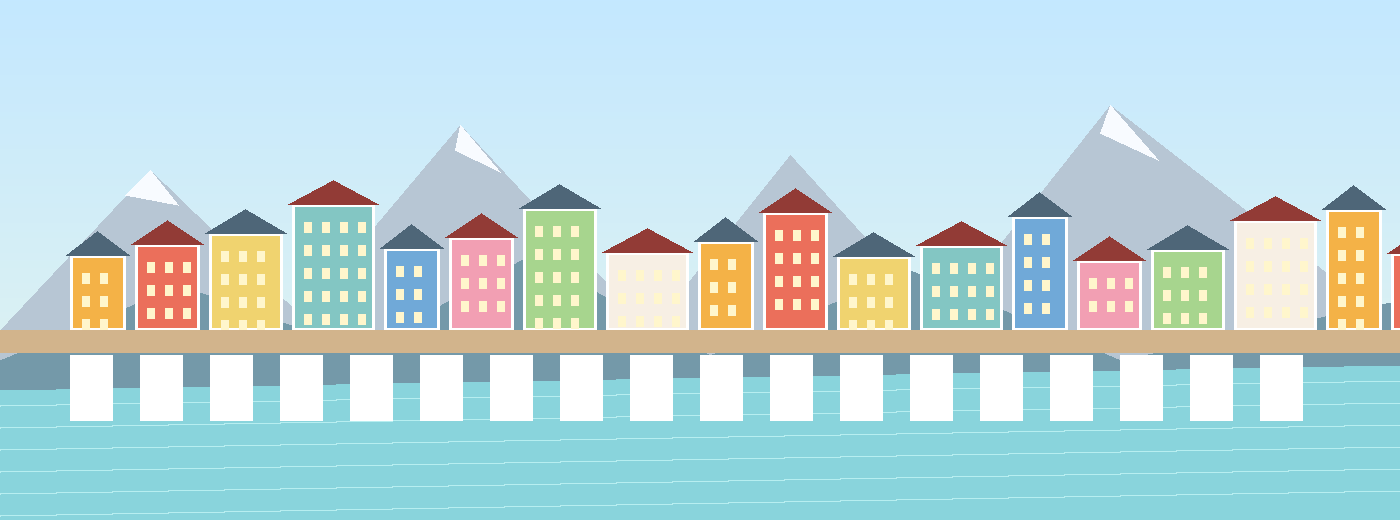
\includegraphics[width=\linewidth]{figures/aurora-landscape.png}
  \caption{A generated landscape used by the template example.}
  \label{fig:aurora-landscape}
\end{figure}
\end{lstlisting}

The command will be presented in prose as follows:

% ------------------------------
%  excerpt box
% ------------------------------
\begin{excerpt}
To see the image, have a look at Figure~\ref{fig:aurora-landscape}.
\end{excerpt}

% ------------------------------
%  figure with included graphic
% ------------------------------
\begin{figure}[H]
  \centering
  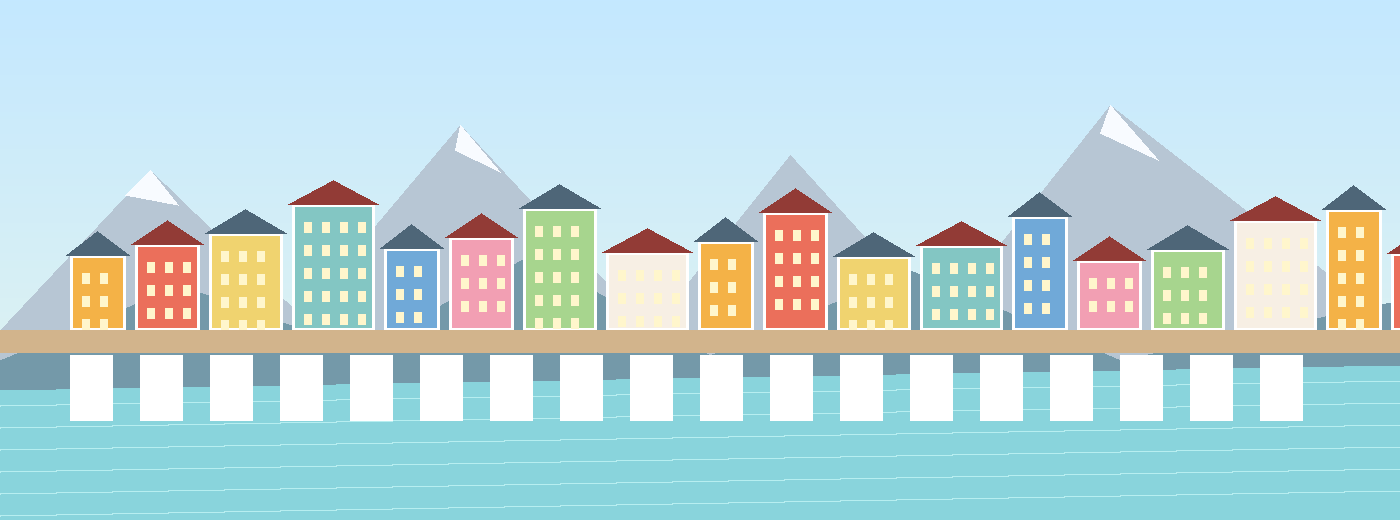
\includegraphics[width=\linewidth]{figures/aurora-landscape.png}
  \caption{A generated landscape used by the template example. The image is
  deliberately stored in the repository so the example compiles without remote
  assets.}
  \label{fig:aurora-landscape}
\end{figure}

\section{Defined Environments}

The template relies on \inlinecode{tcolorbox} for compact, breakable information
boxes. They are intentionally flat: a pale background, a strong left rule, and
no decorative frame.

% ------------------------------
%  excerpt / example / highlight boxes
% ------------------------------
\begin{excerpt}
This is an excerpt box. It is useful for a quotation, a key result, or a short
callout that should remain visually calm.
\end{excerpt}

\begin{example}
This is an example box. Use it when a small idea needs attention without
interrupting the flow of the report.
\end{example}

\begin{highlight}
This is a highlight box for a short reminder or conclusion.
\end{highlight}

% ------------------------------
%  inline highlighting
% ------------------------------
Inline emphasis can use \inlinecode{\textbackslash hlight\{...\}}:
highlighting text is \hlight{very easy} while preserving the surrounding
paragraph style.

% ------------------------------
%  definition environment
% ------------------------------
\begin{definition}
A report template is a reusable document structure that separates layout
decisions from report content.
\end{definition}

% ------------------------------
%  code block (Python example)
% ------------------------------
\begin{lstlisting}[language=Python,style=AuroraListing]
def hello():
    print("Hello, AuroraTeX!")
\end{lstlisting}

\subsection{Writing Equations}

Mathematical content keeps standard LaTeX behavior. Unnumbered equations work
well for quick derivations:

\[
  f(x) = x^2 + 2x + 1
\]

Numbered equations can be referenced in the usual way:

% ------------------------------
%  numbered equation with \label
% ------------------------------
\begin{equation}
  \int_0^1 x^2\,dx = \frac{1}{3}.
  \label{eq:unit-square}
\end{equation}

Equation~\ref{eq:unit-square} is numbered by chapter, matching the report
structure.

\subsection{Designing a Table}

Use \inlinecode{booktabs} for tables. Heavy vertical rules are avoided so the
reader can compare rows quickly.

% ------------------------------
%  table with booktabs + tabularx
% ------------------------------
\begin{table}[H]
  \centering
  \caption{A compact scientific-method table.}
  \label{tab:method}
  \begin{tabularx}{\linewidth}{@{}lXX@{}}
    \toprule
    Section & Scientific method step & Report purpose \\
    \midrule
    Introduction & State the hypothesis & Define scope and motivation \\
    Methods & Describe reproducibility & Explain how results were obtained \\
    Results & Summarize observations & Present data without interpretation \\
    Discussion & Interpret evidence & Connect findings to the hypothesis \\
    \bottomrule
  \end{tabularx}
\end{table}

% ===========================================================================
%  Plotting your data using PGF/TikZ
% ===========================================================================
%  This chapter demonstrates the PGFPlots integration provided by AuroraTeX.
%  It shows both 2D and 3D plots, code snippets, and a description list
%  explaining common axis parameters.
% ===========================================================================

\Chapter{Plotting your data using PGF/TikZ}

\section{Introduction}

PGFPlots and TikZ are useful when the figure should stay editable inside the
source document. The template defines a small \inlinecode{aurora} axis style so
common plots share grid, label, and legend conventions.

% ------------------------------
%  excerpt box
% ------------------------------
\begin{excerpt}
PGF/TikZ describes vector graphics with TeX macros. That makes technical
figures portable, reproducible, and easy to keep visually consistent with the
rest of the report.
\end{excerpt}

\subsection{A Simple 2D Plot}

The following plot compares two functions and is computed by PGFPlots during
compilation.

% ------------------------------
%  2D PGFPlots figure — uses the `aurora` axis style
% ------------------------------
\begin{figure}[H]
  \centering
  \begin{tikzpicture}
    \begin{axis}[
      aurora,
      xlabel={$x$},
      ylabel={$f(x)$},
      domain=-10:10,
      samples=120,
      legend pos=north west
    ]
      \addplot[red, very thick] {x^3 - 7*x - 1};
      \addlegendentry{$x^3 - 7x - 1$}
      \addplot[blue, very thick] {x^2 + 2*x + 1};
      \addlegendentry{$x^2 + 2x + 1$}
    \end{axis}
  \end{tikzpicture}
  \caption{A 2D PGFPlots figure comparing two functions.}
  \label{fig:two-dimensional-plot}
\end{figure}

% ------------------------------
%  code block (LaTeX for the 2D plot)
% ------------------------------
\begin{lstlisting}[language={[LaTeX]TeX},style=AuroraListing]
\begin{axis}[aurora, xlabel={$x$}, ylabel={$f(x)$}]
  \addplot[red, very thick] {x^3 - 7*x - 1};
  \addlegendentry{$x^3 - 7x - 1$}
  \addplot[blue, very thick] {x^2 + 2*x + 1};
  \addlegendentry{$x^2 + 2x + 1$}
\end{axis}
\end{lstlisting}

% ------------------------------
%  description list — axis parameters explained
% ------------------------------
\begin{description}
  \item[domain] The range over which the function is calculated.
  \item[samples] The number of evaluations used to draw the curve.
\end{description}

\subsection{Plotting 3D plots}

Three-dimensional surfaces are also possible with the same axis system. The
example below uses a small sample count so compilation remains fast for a
template repository.

% ------------------------------
%  3D PGFPlots figure — surface plot with colormap
% ------------------------------
\begin{figure}[H]
  \centering
  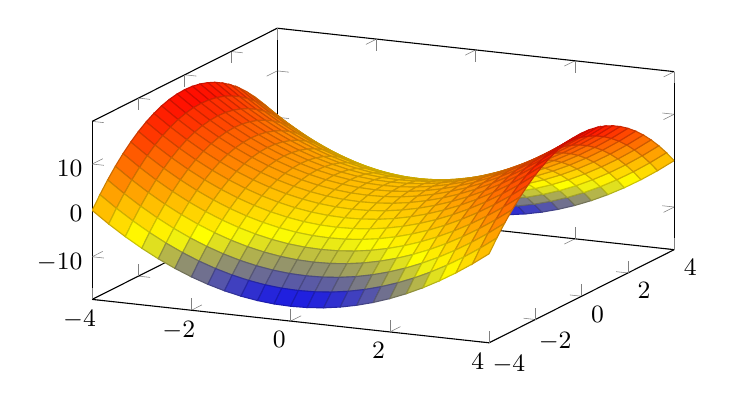
\begin{tikzpicture}
    \begin{axis}[
      view={25}{30},
      width=0.74\textwidth,
      height=0.46\textwidth,
      axis lines=box,
      colormap/hot,
      tick label style={font=\small},
      label style={font=\small}
    ]
      \addplot3[
        surf,
        shader=faceted,
        samples=25,
        domain=-4:4,
        y domain=-4:4
      ] {x^2 - y^2};
    \end{axis}
  \end{tikzpicture}
  \caption{An example 3D plot produced with PGFPlots.}
  \label{fig:three-dimensional-plot}
\end{figure}

% ------------------------------
%  code block (LaTeX for the 3D plot)
% ------------------------------
\begin{lstlisting}[language={[LaTeX]TeX},style=AuroraListing]
\begin{axis}[view={25}{30}, colormap/hot]
  \addplot3[
    surf,
    shader=faceted,
    samples=25,
    domain=-4:4,
    y domain=-4:4
  ] {x^2 - y^2};
\end{axis}
\end{lstlisting}

Because the figures are written as source, color, labels, legends, and data
ranges can be adjusted without replacing external image files.


% --- Bibliography ----------------------------------------------------------
%  \nocite{*} includes every entry in references.bib even if not cited.
%  Replace plainnat with your preferred natbib style (e.g. unsrtnat, abbrvnat).
% ---------------------------------------------------------------------------
\clearpage
\nocite{auroratex,pgfplots}
\bibliographystyle{plainnat}
\bibliography{references}

\end{document}
